\chapter{Red-Black Gauss-Seidel}
\label{cha:gauss-seidel}

\section{Versão 1}
\label{sec:gs-version1}

Esta primeira implementação do método \textit{Red-Black Gauss-Seidel} é bastante simples e direta. Representa-se cada ponto $u(x, y)$ do \textit{grid} em um vetor, como demonstrado na Figura \ref{fig:grid-v1}. Uma função $L(x, y)$ traduz os pontos $x$ e $y$ do \textit{grid} em um índice $i$ do vetor. A avaliação de cada ponto é feita de forma sequencial em \textit{x} e \textit{y} e cada \textit{thread} trabalha sobre um conjunto contínuo na dimensão \textit{x} (conjunto de linhas). Note que como o método Red-Black trabalha primeiramente sobre todos os pontos vermelhos e só então nos pretos, o acesso ao vetor não é estritamente sequencial pois neste os pontos vermelhos e pretos estão intercalados, assim reduzindo o aproveitamento da cache.

\begin{figure}[h]
    \centering
    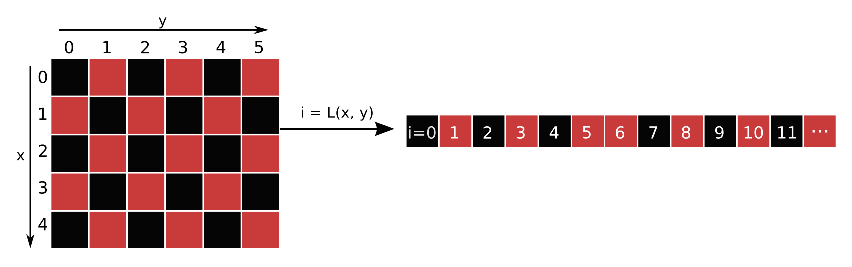
\includegraphics[width=.8\textwidth]{figures/grid-v1}

    \caption{Diagrama do mapeamento do \textit{grid} (à esquerda) em um vetor (à direita) na \textbf{versão 1} do algoritmo.}
    \label{fig:grid-v1}
\end{figure}

Como o cálculo da função $f(x, y)$ é realizado múltiplas vezes para os mesmos pontos, calcula-se previamente uma tabela com os valores de $f(x, y)$ para todo $x$ e $y$. Todos os cálculos da função $f$ reduzem-se à uma consulta à esta tabela.

\begin{figure}[H]
    \centering
    \begin{minipage}{.5\textwidth}
        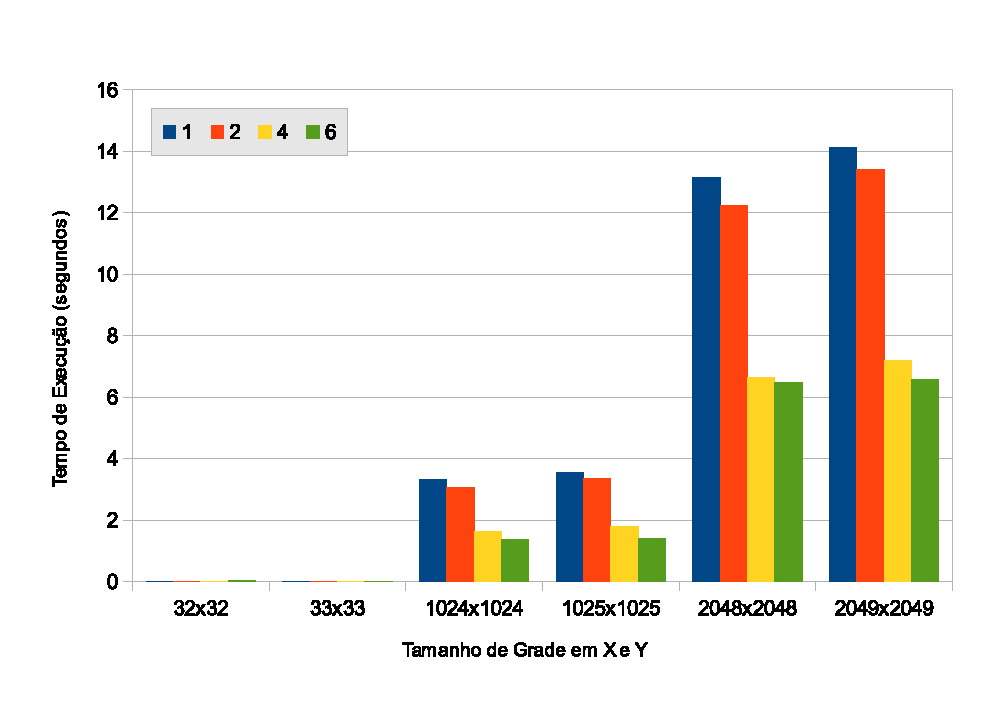
\includegraphics[width=\textwidth]{figures/exectime-v1}
        \subcaption{Tempo de execução}
        \label{subfig:exectime-v1}
    \end{minipage}%
    \begin{minipage}{.5\textwidth}
        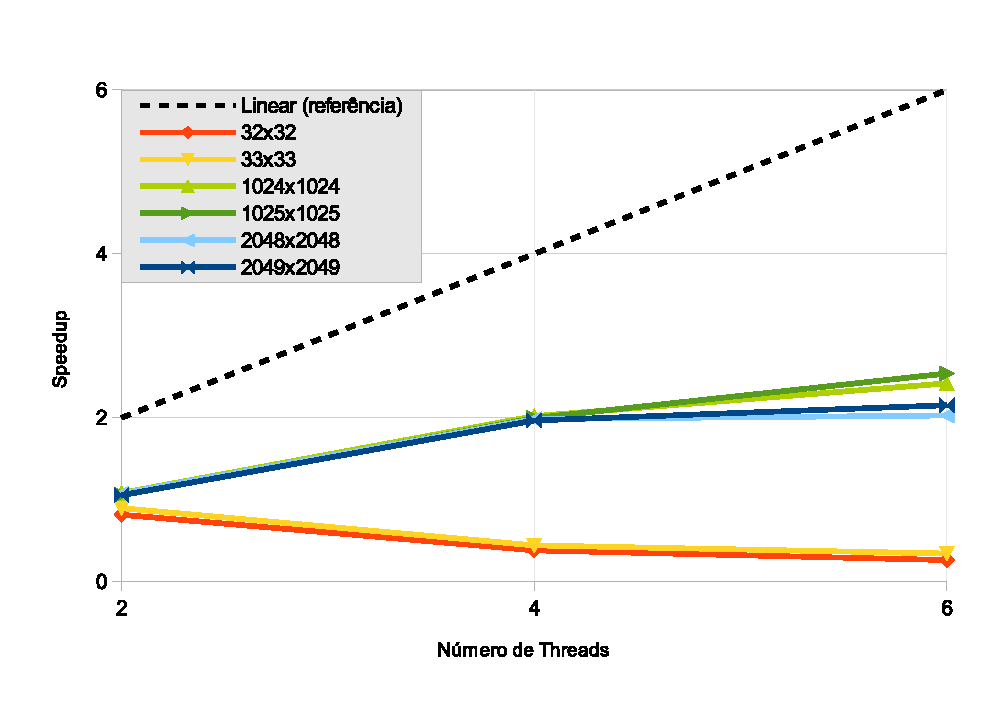
\includegraphics[width=\textwidth]{figures/speedup-v1}
        \subcaption{Speedup}
        \label{subfig:speedup-v1}
    \end{minipage}

    \begin{minipage}{.5\textwidth}
        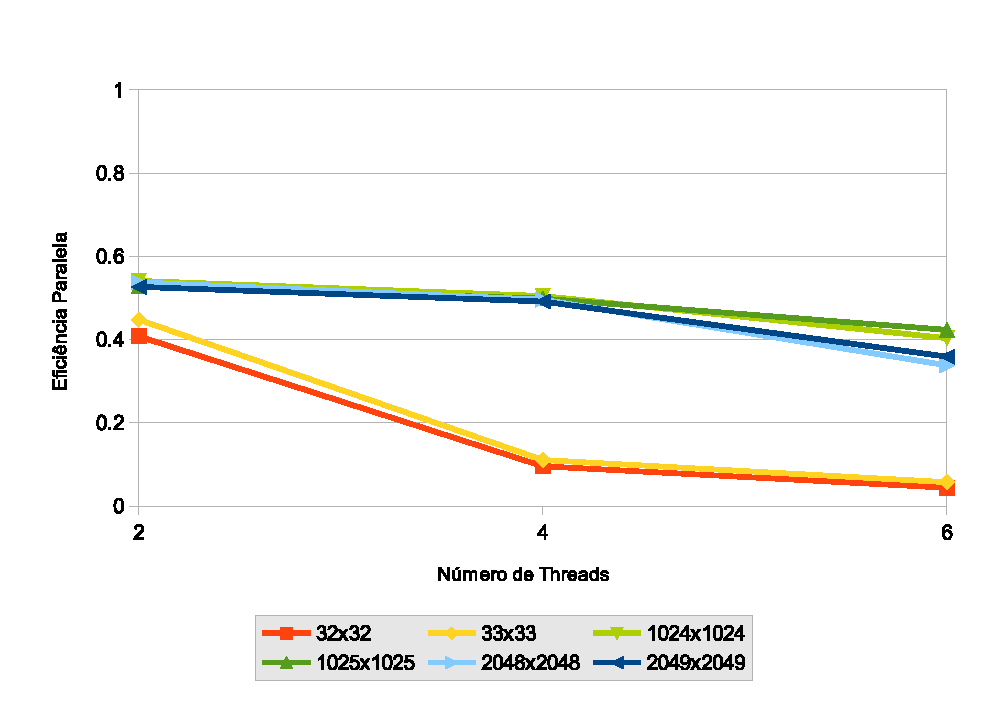
\includegraphics[width=\textwidth]{figures/efficiency-v1}
        \subcaption{Eficiência}
        \label{subfig:efficiency-v1}
    \end{minipage}%

    \caption{Gráficos do tempo de execução (a), \textit{speedup} (b) e eficiência paralela (c) a partir da média de 30 execuções do Red-Black Gauss-Seidel \textbf{versão 1} (200 iterações por execução).}
    \label{fig:perf-v1}
\end{figure}

\section{Versão 2}
\label{sec:gs-version2}

Para fazer melhor uso da \textit{cache}, o \textit{grid} é dividido em dois vetores: \textit{red} e \textit{black}. O primeiro contém todos os pontos vermelhos e o segundo todos os pretos, como na Figura \ref{fig:grid-v2}. Desse modo, a escrita é sempre feita de forma sequencial, visto que o algoritmo percorre o \textit{grid} escrevendo o valor de todos os pontos vermelhos (que agora estão dispostos sequencialmente em um um vetor) e, numa segunda passada, todos os pontos pretos.  A leitura dos valores vizinhos ocorre sempre em três regiões distintas da memória, porém em cada região o acesso é sequencial.

\begin{figure}[h]
    \centering
    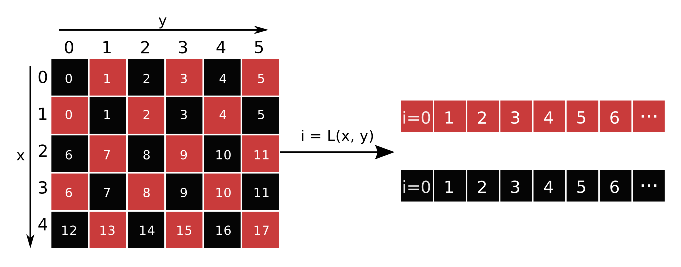
\includegraphics[width=.8\textwidth]{figures/grid-v2}

    \caption{Diagrama do mapeamento do \textit{grid} (à esquerda) em dois vetores \textit{red} e \textit{black} (à direita) na \textbf{versão 2} do algoritmo.}
    \label{fig:grid-v2}
\end{figure}

\begin{figure}[H]
    \centering
    \begin{minipage}{.5\textwidth}
        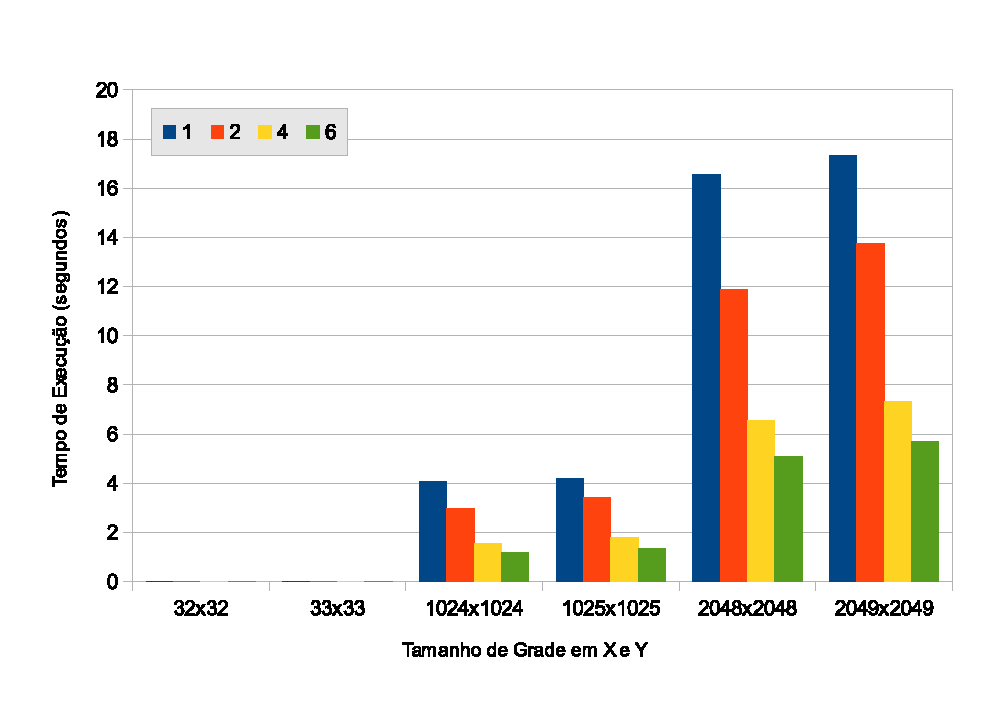
\includegraphics[width=\textwidth]{figures/exectime-v2}
        \subcaption{Tempo de execução}
        \label{subfig:exectime-v2}
    \end{minipage}%
    \begin{minipage}{.5\textwidth}
        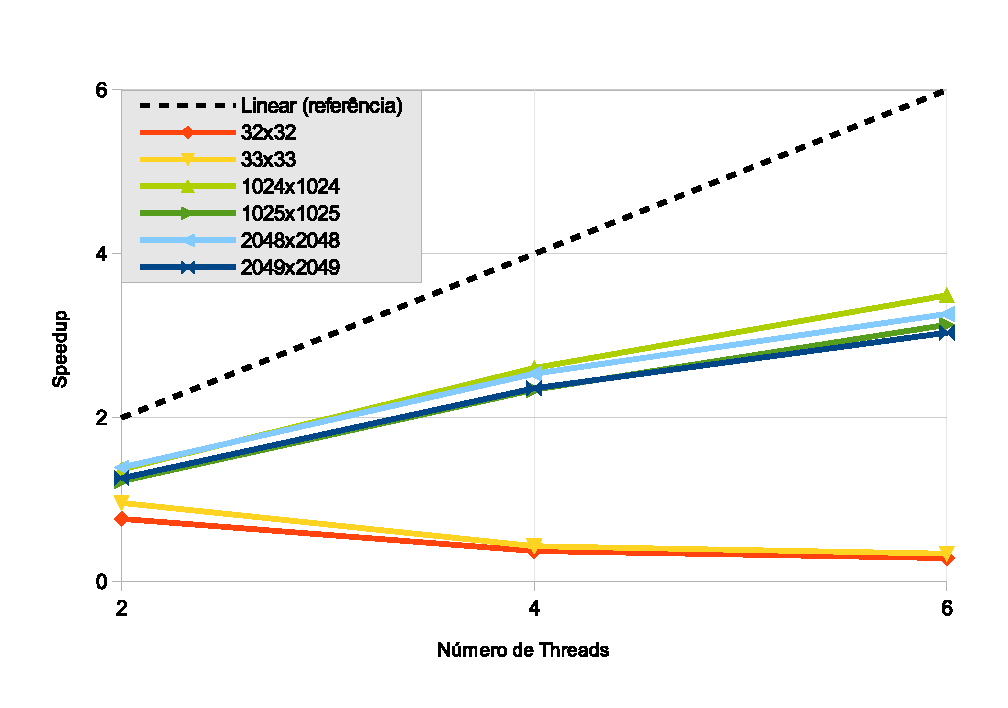
\includegraphics[width=\textwidth]{figures/speedup-v2}
        \subcaption{Speedup}
        \label{subfig:speedup-v2}
    \end{minipage}

    \begin{minipage}{.5\textwidth}
        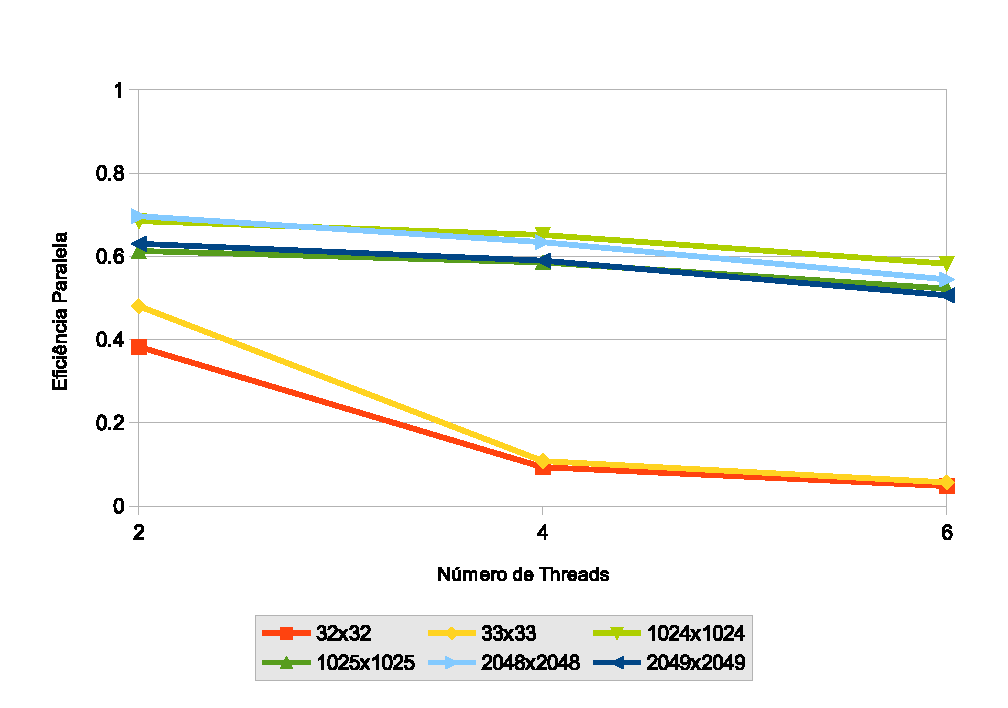
\includegraphics[width=\textwidth]{figures/efficiency-v2}
        \subcaption{Eficiência}
        \label{subfig:efficiency-v2}
    \end{minipage}%

    \caption{Gráficos do tempo de execução (a), \textit{speedup} (b) e eficiência paralela (c) a partir da média de 30 execuções do Red-Black Gauss-Seidel \textbf{versão 2} (200 iterações por execução).}
    \label{fig:perf-v2}
\end{figure}

O resultado dos experimentos (Figura \ref{fig:perf-v2}) mostra que o tempo de execução para 1 ou 2 \textit{threads} nesta versão ficou significativamente mais longo que na anterior. Na primeira versão, o cálculo do índice ($i$) de um ponto $u(x, y)$ na memória (vetorização do \textit{grid}) resume-se ao cálculo de uma simples função $L(x, y)$ contendo um único desvio condicional. Já na segunda versão, essa vetorização é um tanto mais complexa e envolve múltiplos desvios condicionais. Acredito que essa complexidade adicional é responsável pelo pior desempenho desse.

No entanto, o \textit{speedup} apresenta-se melhor nessa versão ao ponto de que para 4 ou mais \textit{threads} o tempo de execução é menor do que na versão 1.


\section{Versão 3}
\label{sec:gs-version3}

O compilador GCC provém uma forma de representar dados para que as operações executadas sobre estes possam ser -- explicitamente -- executadas por instruções SIMD (MMX, 3DNow! ou SSE no caso de processadores i386). Esta representação é denominada \textit{Vector Extensions} \cite{vectorextensions}. Dessa forma, podemos representar dois números do tipo \textit{double} em uma única variável (ou posição em um vetor) e todas as operações efetuadas sobre estes serão feitas para ambos os números numa mesma instrução SIMD.

Com isso em mente, podemos representar em uma única posição de um vetor o valor de dois pontos (Figura \ref{fig:grid-v3}) e, também, efetuar o cálculo de seus valores ao mesmo tempo. Logo, o tamanho de cada um dos vetores (em número de posições, não em número de pontos) é reduzido pela metade e o número de instruções a serem executadas também.

\begin{figure}[h]
    \centering
    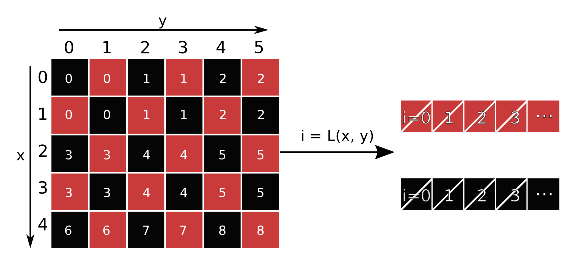
\includegraphics[width=.8\textwidth]{figures/grid-v3}

    \caption{Diagrama do mapeamento do \textit{grid} (à esquerda) em dois vetores \textit{red} e \textit{black} onde cada posição armazena dois pontos (à direita) na \textbf{versão 3} do algoritmo.}
    \label{fig:grid-v3}
\end{figure}

Como mostra a Figura \ref{fig:grid-calc}, o cálculo é feito simultaneamente para dois pontos que têm dois vizinhos em comum no \textit{stencil} reduzindo o acesso à memória em geral. Note também que o acesso aos vetores continua sendo sequencial -- como na versão anterior -- fazendo bom uso da cache. Ao contrário da versão anterior, o cálculo do índice ($i$) de uma dupla de pontos consecutivos é simples e envolve apenas duas operações aritméticas (nenhum desvio condicional).

\begin{figure}[h]
    \centering
    \begin{minipage}{.6\textwidth}
    \includegraphics[width=.9\textwidth]{figures/grid-calc}
    \end{minipage}%
    \begin{minipage}{.4\textwidth}
    \caption{Exemplo de cálculo de dois pontos na \textbf{versão 3} do Red-Black Gauss-Seidel. Os dois pontos que estão localizados no índice 4 do vetor preto são calculados simultaneamente. Note que os dois pontos vermelhos de índice 4 são vizinhos no \textit{stencil} de ambos os pontos pretos e, logo, para sua leitura é necessário apenas uma busca na memória. Se os pontos pretos fossem calculados individualmente como nas versões anteriores, duas buscas na memória se fazem necessárias (uma leitura para cada ponto preto).}
    \label{fig:grid-calc}
    \end{minipage}%
\end{figure}

A leitura dos pontos $u(x, y+1)$ e $u(x+1, y)$ (ambos necessários para o cálculo do ponto $u(x, y)$) podem, dependendo do tamanho da dimensão $y$, coincidir na mesma posição da cache ocasionando aumento de \textit{cache misses}. Esse problema é conhecido como \textit{cache thrashing} \cite{cachethrashing} e para evitá-lo adiciona-se um \textit{padding}, ou seja, posições vazias na dimensão $y$ a fim de que as posições acessadas não caiam na mesma posição da cache. A Figura \ref{fig:padding} mostra a razão entre \textit{cache misses} e \textit{cache access} para diversos tamanho de \textit{grid} e tamanhos de \textit{padding}. O tamanho de \textit{padding} escolhido foi 16 já que este apresenta o menor número de \textit{cache misses} e acima deste valor não é apresentado nenhum ganho.

\begin{figure}[h]
    \centering
    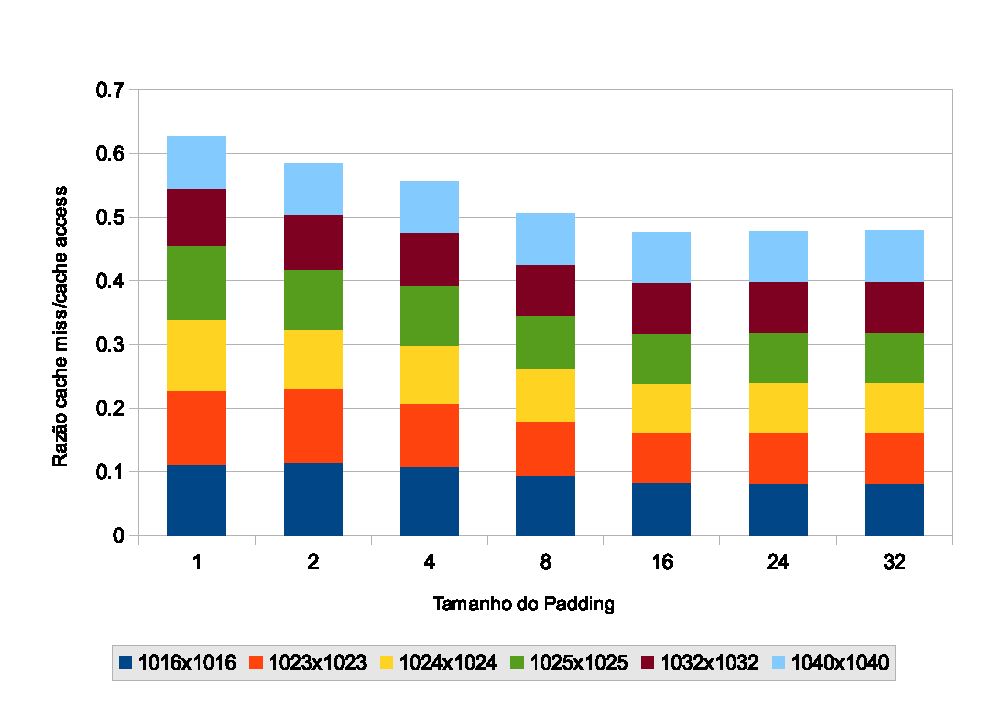
\includegraphics[width=.8\textwidth]{figures/padding}

    \caption{Gráfico da razão entre \textit{cache misses} e \textit{cache access} para diversos tamanho de \textit{grid} e tamanhos de \textit{padding}.}
    \label{fig:padding}
\end{figure}


\begin{figure}[H]
    \centering
    \begin{minipage}{.5\textwidth}
        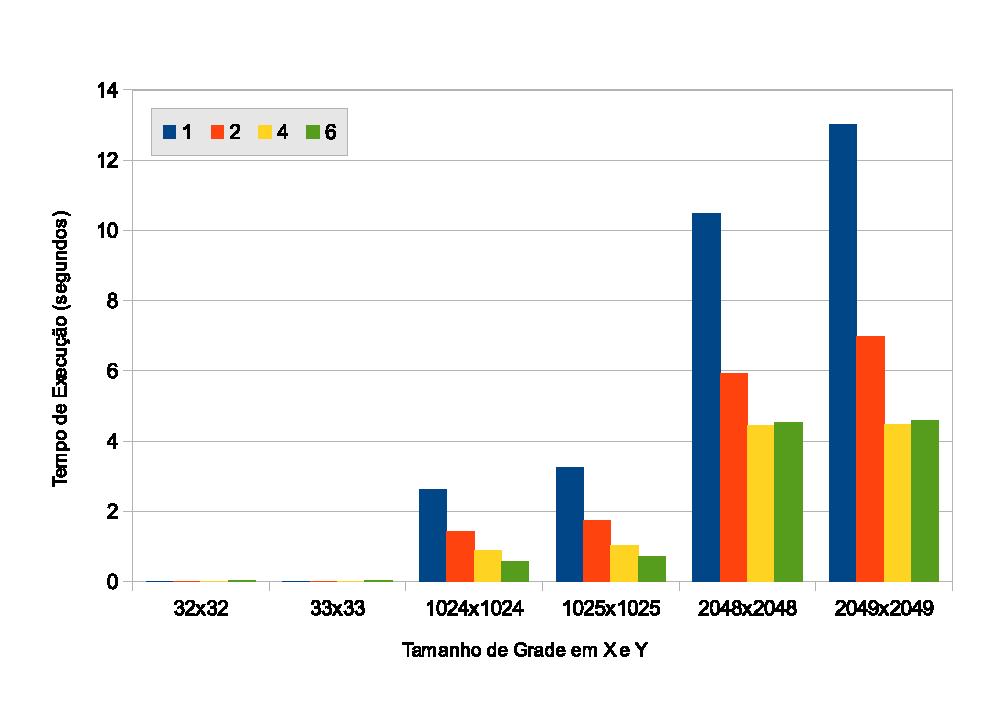
\includegraphics[width=\textwidth]{figures/exectime-v3}
        \subcaption{Tempo de execução}
        \label{subfig:exectime-v3}
    \end{minipage}%
    \begin{minipage}{.5\textwidth}
        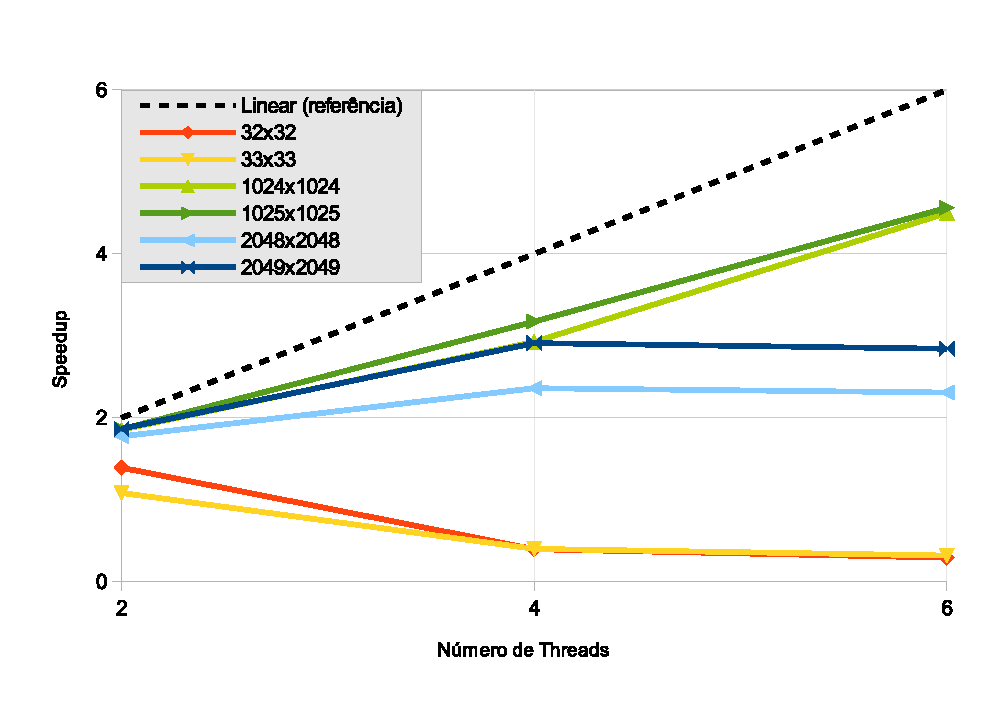
\includegraphics[width=\textwidth]{figures/speedup-v3}
        \subcaption{Speedup}
        \label{subfig:speedup-v3}
    \end{minipage}

    \begin{minipage}{.5\textwidth}
        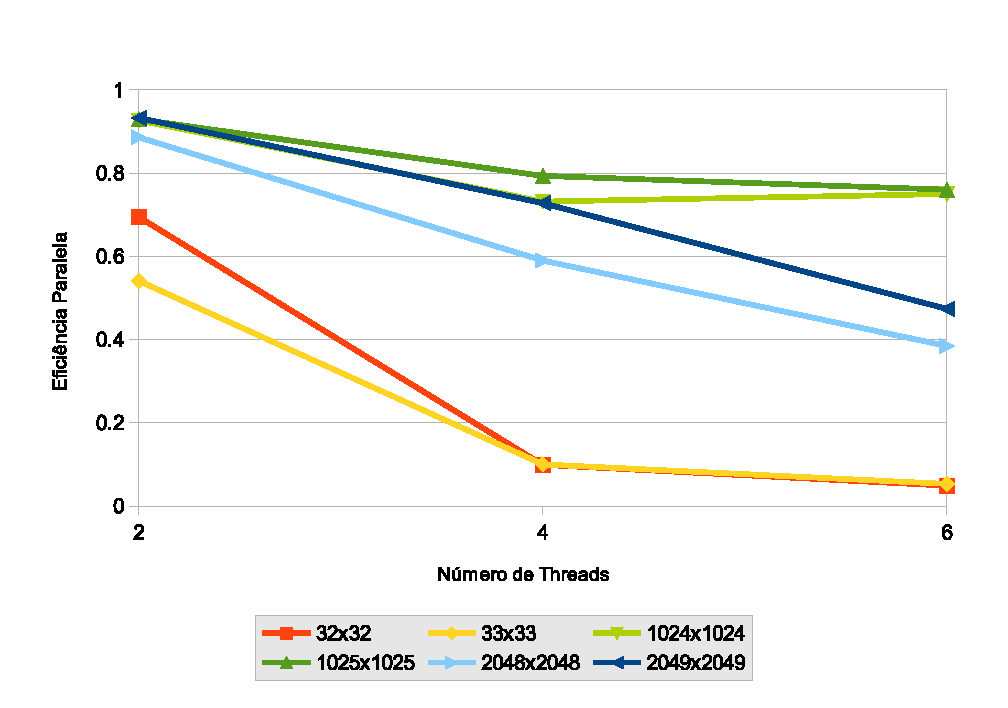
\includegraphics[width=\textwidth]{figures/efficiency-v3}
        \subcaption{Eficiência}
        \label{subfig:efficiency-v3}
    \end{minipage}%

    \caption{Gráficos do tempo de execução (a), \textit{speedup} (b) e eficiência paralela (c) a partir da média de 30 execuções do Red-Black Gauss-Seidel \textbf{versão 3} (200 iterações por execução).}
    \label{fig:perf-v3}
\end{figure}

Todos esses fatores apresentados levam a um tempo de execução -- para todos os tamanhos de grade -- menor do que as versões anteriores (Figura \ref{subfig:exectime-v3}). A eficiência paralela também demonstra-se melhor nessa versão (Figura \ref{subfig:efficiency-v3}).